\begin{knitrout}\scriptsize
\definecolor{shadecolor}{rgb}{0.969, 0.969, 0.969}\color{fgcolor}\begin{figure}[H]

{\centering \includegraphics[width=1\linewidth]{figure/toy-solution-path-1} 

}

\caption[Toy example solution path for main effects (top) and interactions (bottom)]{Toy example solution path for main effects (top) and interactions (bottom). $\left\lbrace X1_1, X1_2, X1_3 \right\rbrace$ and $\left\lbrace X2_1, X2_2, X2_3 \right\rbrace$ are the three basis coefficients for $X_1$ and $X_2$, respectively. $\lambda_{1SE}$ is the largest value of penalization for which the CV error is within one standard error of the minimizing value $\lambda_{min}$.}\label{fig:toy-solution-path}
\end{figure}
\end{knitrout}

\begin{knitrout}\scriptsize
	\definecolor{shadecolor}{rgb}{0.969, 0.969, 0.969}\color{fgcolor}\begin{figure}[H]
		
		{\centering \includegraphics[width=1\linewidth]{figure/toy-effects-1} 
			
		}
		
		\caption[Estimated smooth functions for $X_1$ and the $X_2 \cdot E$ interaction by the \texttt{sail} method based on $\lambda_{min}$]{Estimated smooth functions for $X_1$ and the $X_2 \cdot E$ interaction by the \texttt{sail} method based on $\lambda_{min}$.}\label{fig:toy-effects}
	\end{figure}
	
	
\end{knitrout}


\begin{knitrout}\scriptsize
	\definecolor{shadecolor}{rgb}{0.969, 0.969, 0.969}\color{fgcolor}\begin{figure}[h]
		
		{\centering \includegraphics[width=1\linewidth]{figure/plot-mse-sim-1} 
			
		}
		
		\caption[Boxplots of the test set mean squared error from 200 simulations for each of the five simulation scenarios]{Boxplots of the test set mean squared error from 200 simulations for each of the five simulation scenarios.}\label{fig:plot-mse-sim}
	\end{figure}
	
	
\end{knitrout}



% this is only commented because i dont want to change the paths to figures
% for carbon laptop
%\begin{comment}
\begin{figure}[h]
	\centering
	\includegraphics[scale=0.61]{/home/sahir/git_repositories/sail/my_sims/figures/sail_main_eff_paramIndex1_200sims.pdf}
	\caption{True and estimated main effect component functions for scenario 1a). The estimated curves represent the results from each one of the 200 simulations conducted.}\label{fig:main_eff}
\end{figure}


\begin{figure}[h]
	\centering
	\subfloat{\includegraphics[width=0.37\linewidth]{/home/sahir/git_repositories/sail/my_sims/figures/sail_intertruth_X3_paramIndex1_200sims.pdf}}
	\subfloat{\includegraphics[width=0.37\linewidth]{/home/sahir/git_repositories/sail/my_sims/figures/sail_inter25_X3_paramIndex1_200sims.pdf}}\quad
	\subfloat{\includegraphics[width=0.37\linewidth]{/home/sahir/git_repositories/sail/my_sims/figures/sail_inter50_X3_paramIndex1_200sims.pdf}}
	\subfloat{\includegraphics[width=0.37\linewidth]{/home/sahir/git_repositories/sail/my_sims/figures/sail_inter75_X3_paramIndex1_200sims.pdf}}
	\caption{True and estimated interaction effects for $X_E \cdot f_3(X_3)$ in simulation scenario 1a).}
	\label{fig:X3}
\end{figure}


\begin{figure}[h]
	\centering
	\subfloat{\includegraphics[width=0.37\linewidth]{/home/sahir/git_repositories/sail/my_sims/figures/sail_intertruth_X4_paramIndex1_200sims.pdf}}
	\subfloat{\includegraphics[width=0.37\linewidth]{/home/sahir/git_repositories/sail/my_sims/figures/sail_inter25_X4_paramIndex1_200sims.pdf}}\quad
	\subfloat{\includegraphics[width=0.37\linewidth]{/home/sahir/git_repositories/sail/my_sims/figures/sail_inter50_X4_paramIndex1_200sims.pdf}}
	\subfloat{\includegraphics[width=0.37\linewidth]{/home/sahir/git_repositories/sail/my_sims/figures/sail_inter75_X4_paramIndex1_200sims.pdf}}
	\caption{True and estimated interaction effects for $X_E \cdot f_4(X_4)$ in simulation scenario 1a).}
	\label{fig:X4}
\end{figure}


\begin{knitrout}\scriptsize
	\definecolor{shadecolor}{rgb}{0.969, 0.969, 0.969}\color{fgcolor}\begin{figure}[h]
		
		{\centering \includegraphics[width=1\linewidth]{figure/PRS-intervention-interaction-1} 
			
		}
		
		\caption[Estimated interaction effect identified by the weak heredity \texttt{sail} using cubic B-splines and $\alpha=0.1$ for the Nurse Family Partnership data]{Estimated interaction effect identified by the weak heredity \texttt{sail} using cubic B-splines and $\alpha=0.1$ for the Nurse Family Partnership data. The selected model, chosen via 10-fold cross-validation, contained three variables: the main effects for the intervention and the PRS for educational attainment using genetic variants significant at the 0.0001 level, as well as their interaction.}\label{fig:PRS-intervention-interaction}
	\end{figure}
	
	
\end{knitrout}



\begin{knitrout}\scriptsize
	\definecolor{shadecolor}{rgb}{0.969, 0.969, 0.969}\color{fgcolor}\begin{figure}[h]
		
		{\centering 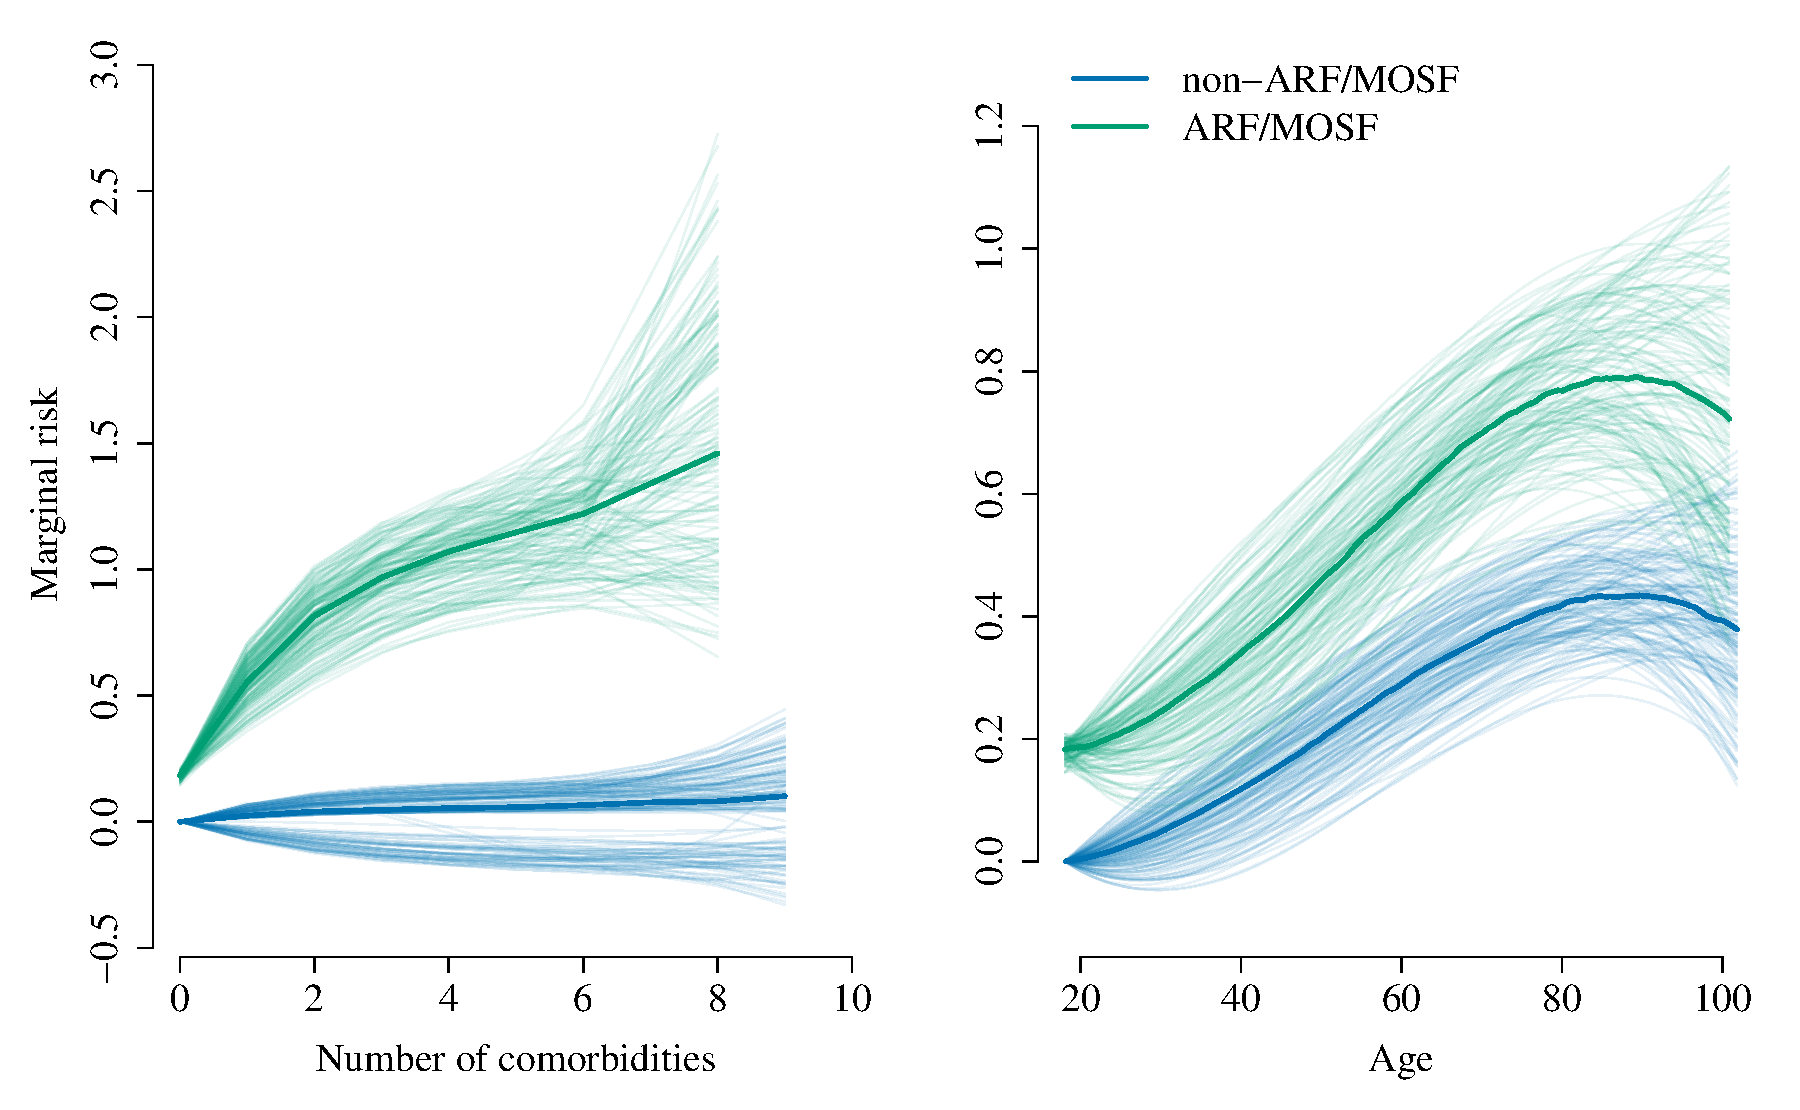
\includegraphics[width=1\linewidth]{figure/dzclass-interaction-1} 
			
		}
		
		\caption[Illustration of estimated interaction effects identified by \texttt{sail} for the SUPPORT data]{Illustration of estimated interaction effects identified by \texttt{sail} for the SUPPORT data. Median prediction curves in dark colors based on 200 train/validate/test splits represent the estimated marginal interaction effects. Coefficients estimated in each of the 200 train/validate/test splits were used to generate prediction curves representing a 90\% confidence interval colored in corresponding light colors.}\label{fig:dzclass-interaction}
	\end{figure}
	
	
\end{knitrout}